\documentclass[conference]{IEEEtran}
\usepackage{amsmath,amssymb,graphicx,booktabs,multirow,xcolor,tikz,cite,url}
\usetikzlibrary{arrows.meta,positioning,fit,backgrounds}
\newcommand{\ours}{\textsc{MS}}
\begin{document}

\title{A Low-Cost Closed-Loop MLOps Pipeline with AutoML and Multi-Signal Drift Alerting on Serverless Cloud}

\author{
\IEEEauthorblockN{Prajna}
\IEEEauthorblockA{\textit{School of CSE}\\
\textit{RV University}\\
Bengaluru, India\\
1RVU23CSE339}
\and
\IEEEauthorblockN{Nandan Kumar S}
\IEEEauthorblockA{\textit{School of CSE}\\
\textit{RV University}\\
Bengaluru, India\\
1RVU23CSE299}
\and
\IEEEauthorblockN{Dr. Revansiddappa}
\IEEEauthorblockA{\textit{Associate Professor}\\
\textit{School of CSE}\\
\textit{RV University}\\
Bengaluru, India}
}

\maketitle

\begin{abstract}
Deployed machine-learning models degrade silently as data shifts, yet most pipelines either retrain on a fixed schedule or alert on raw statistical tests that fire on harmless shifts. We present an end-to-end, open-source MLOps loop that joins AutoML model selection (FLAML), a FastAPI prediction service designed for AWS Lambda, an S3-backed model registry and inference log, a scheduled drift job, and CI/CD-triggered retraining with a deployment gate and zero-downtime hot-swap. Its core is a model-agnostic, label-free \emph{multi-signal} drift detector that raises a retrain alarm only when at least two of three signals---input-feature shift, prediction-distribution shift, and confidence drop---agree over consecutive windows. In 20-seed controlled experiments, single-test KS and PSI detectors alarmed on 100\% of windows after a benign shift in features the model ignores, while the multi-signal detector alarmed on 2\%, and still caught 90--95\% of harmful shifts that cut accuracy by 8--17 points within about one window. On the real Elec2 electricity stream, a static model fell from 83.6\% hold-out accuracy to 67.8\%; retraining triggered by our detector recovered 74.4\%, matching KS- and PSI-triggered retraining within run-to-run variation while using 19\% fewer retrains. A live HTTP replay of 20{,}000 records ran nine detect--retrain cycles and six gated redeployments without a restart, with a median of 6.5\,s from alarm to serving and 76.2\% accuracy against 68.0\% for the static model. Deployed on AWS (Lambda, API Gateway, S3, CloudWatch) with one SAM template, the same loop detected drift in live traffic, retrained inside Lambda in 13\,s and promoted a new model (83.0\% vs.\ 78.8\%) that the API served without a redeploy. Lambda and CloudWatch use stays within AWS always-free allowances.
\end{abstract}

\begin{IEEEkeywords}
MLOps, AutoML, concept drift, data drift, model monitoring, serverless, AWS Lambda, CI/CD, continuous training
\end{IEEEkeywords}

\section{Introduction}
A model in production is a living system: it must be served, versioned, watched and replaced as the data it sees moves away from the data it was trained on~\cite{sculley2015}. Vela \emph{et al.} found temporal degradation in 91\% of 128 model--dataset pairs across four industries~\cite{vela2022}. Because labels usually arrive late, degradation must be detected from inputs and predictions alone, and the response---retraining and redeployment---should be automatic~\cite{kreuzberger2023}.

Our literature review of ten recent works exposed three gaps. \emph{(G1)} No surveyed system closes the full loop of AutoML selection, live serving, drift detection, alerting and CI/CD redeployment within a free-tier budget; existing options are paid managed services~\cite{nigenda2022} or isolated components~\cite{garg2021,zoller2021,baier2021}. \emph{(G2)} Statistical detectors flag every significant shift, including shifts that do not affect accuracy~\cite{eck2022}, while uncertainty-based detectors require a specific model family~\cite{baier2021}. \emph{(G3)} Few open experiments measure detection behaviour and recovery on a live prediction API.

\textbf{Contributions.} (1) An open-source closed-loop pipeline---AutoML, serving, logging, drift job, gated retraining, hot-swap---with a validated AWS SAM template and GitHub Actions workflows that keep the cloud footprint within always-free limits. (2) A model-agnostic, label-free multi-signal detector with voting and persistence. (3) A reproducible evaluation on controlled drift with ground truth, the real Elec2 stream, and a live HTTP service.

\section{Related Work}
\textbf{MLOps.} Kreuzberger \emph{et al.}~\cite{kreuzberger2023} define MLOps around CI/CD, versioning, continuous training and monitoring; a multivocal review of 198 sources~\cite{eken2024} reports that cost and complexity push small teams back to manual workflows. Garg \emph{et al.}~\cite{garg2021} map GitOps push/pull deployment onto ML but do not address drift-triggered retraining.
\textbf{AutoML.} AutoML solves the combined algorithm selection and hyper-parameter optimisation (CASH) problem~\cite{he2021}. A benchmark on 73 datasets found all frameworks beat a random-forest baseline with at most 2.2\% spread among them, but none considers deployment or lifecycle~\cite{zoller2021}. We use FLAML for its cost-frugal search and warm-start support~\cite{wang2021flaml}.
\textbf{Drift detection.} Error-rate detectors such as ADWIN~\cite{bifet2007} need labels~\cite{gama2014}. Two-sample tests on inputs are label-free but sensitive to irrelevant shift~\cite{rabanser2019}: Eck \emph{et al.} observed significant feature drift with stable accuracy in a deployed supply-chain system~\cite{eck2022}. Uncertainty Drift Detection~\cite{baier2021} suppresses such alarms but needs a dropout neural network.
\textbf{Monitoring and retraining.} SageMaker Model Monitor~\cite{nigenda2022} detects several drift types at scale but stops at the alert and is a paid service. Katalay \emph{et al.}~\cite{katalay2025} combine statistical criteria to trigger retraining of neural classifiers, evaluated offline on anomaly-detection benchmarks.

\section{System Design}
\begin{figure}[t]
\centering
\resizebox{\columnwidth}{!}{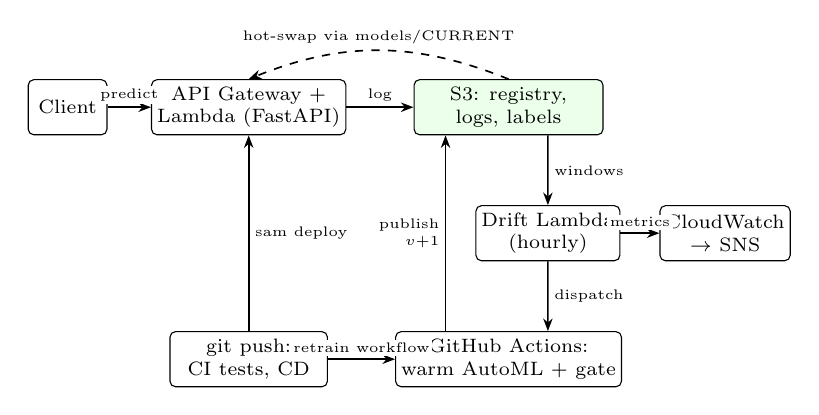
\begin{tikzpicture}[font=\scriptsize,
  b/.style={draw, rounded corners=2pt, align=center, minimum height=7mm, inner sep=2pt, fill=white},
  a/.style={-{Stealth[length=1.6mm]}, semithick}, l/.style={font=\tiny, fill=white, inner sep=1pt}]
\node[b, minimum width=10mm] (cli) at (0,0) {Client};
\node[b, minimum width=20mm] (api) at (2.3,0) {API Gateway +\\Lambda (FastAPI)};
\node[b, minimum width=24mm, fill=green!8] (s3) at (5.6,0) {S3: registry,\\logs, labels};
\node[b, minimum width=14mm] (drift) at (6.1,-1.6) {Drift Lambda\\(hourly)};
\node[b, minimum width=12mm] (cw) at (8.35,-1.6) {CloudWatch\\$\rightarrow$ SNS};
\node[b, minimum width=24mm] (gha) at (5.6,-3.2) {GitHub Actions:\\warm AutoML + gate};
\node[b, minimum width=20mm] (dev) at (2.3,-3.2) {git push:\\CI tests, CD};
\draw[a] (cli) -- node[l, above=1pt]{predict} (api);
\draw[a] (api) -- node[l, above=1pt]{log} (s3);
\draw[a] ([xshift=5mm]s3.south) -- node[l, right=1pt]{windows} ([xshift=0mm]drift.north);
\draw[a] (drift) -- node[l, above=1pt]{metrics} (cw);
\draw[a] (drift.south) -- node[l, right=1pt]{dispatch} ([xshift=5mm]gha.north);
\draw[a] ([xshift=-8mm]gha.north) -- node[l, left=1pt, align=right]{publish\\$v{+}1$} ([xshift=-8mm]s3.south);
\draw[a, dashed] (s3.north) to[bend right=22] node[l, above=1pt]{hot-swap via models/CURRENT} (api.north);
\draw[a] (dev) -- node[l, above=1pt]{retrain workflow} (gha);
\draw[a] (dev) -- node[l, right=1pt]{sam deploy} (api);
\end{tikzpicture}}
\caption{Closed-loop architecture. Models are data in S3; a new version reaches the running API through an atomic pointer swap, with no redeploy.}
\label{fig:arch}
\end{figure}

Fig.~\ref{fig:arch} shows the loop. Every component reads and writes through one storage interface with a local-directory and an S3 back end, so experiments and the cloud deployment share the same code.

\textbf{AutoML.} FLAML searches LightGBM, XGBoost, random forest, extra trees and $\ell_1$ logistic regression with a fixed time budget and a time-ordered hold-out. Retraining is \emph{warm-started} from the previous best configuration of each learner, which lets a short budget (6--8\,s) give a competitive model.

\textbf{Serving and logging.} A FastAPI service exposes \texttt{/predict}, \texttt{/feedback} (delayed labels) and \texttt{/health}. It runs under uvicorn locally and on Lambda via Mangum in a container image. Each request is logged to S3 with a globally ordered id. The service re-reads the registry pointer \texttt{models/CURRENT} every $R$ seconds and hot-swaps to a newer version; because the pointer is written last, readers never see a half-written version.

\textbf{Multi-signal drift detection.} For a reference window $\mathcal{R}$ (held-out data and the serving model's predictions on it) and a live window $\mathcal{W}$ of $n{=}500$ records with $d$ features, we compute three label-free signals:
\begin{itemize}
\item $S_\text{in}$: the share of features that are shifted under \emph{both} a Bonferroni-corrected KS test ($p < 0.05/d$) and $\text{PSI} > 0.2$ is at least $1/4$, where
$\text{PSI}=\sum_{k}(c_k-r_k)\ln(c_k/r_k)$ over ten reference-quantile bins.
\item $S_\text{pred}$: PSI of the predicted-probability distribution exceeds $0.1$.
\item $S_\text{conf}$: mean confidence $|2\hat p-1|$ drops by more than $0.05$.
\end{itemize}
A window votes ``drift'' when at least two signals fire; an alarm needs two consecutive drift votes, followed by a two-window cooldown. Since $S_\text{in}$ alone can never alarm, shifts in features the model does not use are suppressed, while shifts that move the model's outputs are caught. The rule uses only inputs and outputs, so it applies to whatever model AutoML selects.

\textbf{Retraining and deployment gate.} On alarm, the drift Lambda retrains in place; optionally it can instead send a GitHub \texttt{repository\_dispatch} so that a GitHub Actions workflow retrains. Either path takes the 3{,}000 most recent labelled records, runs warm-started AutoML on the older 80\%, and promotes the candidate only if it matches or beats the serving model on the newest 20\%. The winner is refit on all fresh data and published as version $v{+}1$ together with a new out-of-sample reference window. CI runs unit and end-to-end tests plus \texttt{cfn-lint}; CD builds the image and runs \texttt{sam deploy} using GitHub OIDC, so no long-lived keys are stored.

\textbf{Cost.} The design uses two Lambda functions, one HTTP API, one S3 bucket, three custom metrics and one alarm. AWS's always-free tier covers 1M Lambda requests and 400{,}000\,GB-s per month and 10 custom CloudWatch metrics and alarms~\cite{awsfree}; an hourly drift job at 2\,GB for 20\,s uses about 28{,}800\,GB-s per month. Both functions ship as one container image; using the CPU-only XGBoost build keeps the CUDA libraries (about 500\,MB) out of it. S3, API Gateway and ECR are billed against the sign-up credits AWS gives accounts opened after July 2025.

\section{Experimental Setup}
\textbf{Data.} \emph{Controlled:} a synthetic tabular task (\texttt{make\_classification}, 14{,}000 rows, 8 features of which 4 are informative and 4 are pure noise), so the effect of every shift is known. \emph{Real:} Elec2~\cite{harries1999}, 45{,}312 half-hourly records of the Australian NSW electricity market, label = price up/down, with 7 features (date index dropped). Elec2 is a standard real-world drift benchmark~\cite{gama2014}.

\textbf{Detectors.} KS: Bonferroni-corrected per-feature KS test (practice in~\cite{eck2022}). PSI: any feature $\text{PSI}>0.2$. \ours: ours. Ablations: \ours{} with one vote (logical OR) and without persistence. ErrorRate: alarm when window accuracy falls 5 points below the post-training value; it needs true labels at check time, so it is a supervised reference, not a deployable label-free option.

\textbf{Exp.~1 (controlled, 20 seeds).} Per seed, AutoML (8\,s) trains on 3{,}000 rows; 1{,}000 held-out rows form the reference; 30 windows of 300 rows follow, with drift injected from window 15: \emph{benign} (all four noise features shifted by 1$\sigma$ or 2$\sigma$), \emph{harmful} (two informative features shifted by 0.3, 0.6 or 1.0$\sigma$), or \emph{concept} (30\% of labels flipped, $P(X)$ unchanged). No retraining, to isolate detection.

\textbf{Exp.~2 (Elec2, 3 runs).} Initial AutoML (30\,s) on rows 0--2{,}999, reference on 3{,}000--3{,}999; the next 41{,}000 rows arrive in 82 windows of 500 (test-then-train). Labels lag by one window. Every strategy uses the same warm-started retrain (6\,s budget, 3{,}000 freshest labels) and gate, plus a two-window cooldown for triggered strategies.

\textbf{Exp.~3 (live service).} The FastAPI service runs under uvicorn; 20{,}000 Elec2 rows (4{,}000--23{,}999) are sent as 400 HTTP requests of 50 rows, labels are posted to \texttt{/feedback} one window late, and the drift job runs every 500 rows, retrains in-process and publishes to the registry while the server keeps running. Hardware: a 2-vCPU Linux container; Python 3.13, FLAML 2.7, LightGBM 4.7, XGBoost 2.1.

\section{Results}
\subsection{Benign versus harmful drift (Exp.~1)}
\begin{table}[t]
\caption{Controlled drift, 20 seeds: share of post-drift windows alarmed (benign: lower is better; harmful: higher is better). Accuracy change after drift in brackets.}
\label{tab:ctrl}
\centering\footnotesize\setlength{\tabcolsep}{3pt}
\begin{tabular}{lccccc}
\toprule
 & \multicolumn{2}{c}{Benign} & \multicolumn{3}{c}{Harmful} \\
\cmidrule(lr){2-3}\cmidrule(lr){4-6}
Detector & 1.0$\sigma$ & 2.0$\sigma$ & 0.3$\sigma$ & 0.6$\sigma$ & 1.0$\sigma$ \\
 & {\scriptsize($-$0.1)} & {\scriptsize($-$0.3)} & {\scriptsize($-$2.2)} & {\scriptsize($-$7.8)} & {\scriptsize($-$16.6)} \\
\midrule
KS & 1.00 & 1.00 & 0.99 & 1.00 & 1.00 \\
PSI & 1.00 & 1.00 & 0.41 & 1.00 & 1.00 \\
\ours{} 1-vote (OR) & 0.93 & 0.93 & 0.27 & 0.93 & 0.93 \\
\ours{} no persistence & 0.10 & 0.47 & 0.05 & 0.86 & 0.95 \\
\textbf{\ours{} (full)} & \textbf{0.02} & \textbf{0.36} & 0.02 & 0.76 & 0.88 \\
\midrule
ErrorRate (labels) & 0.00 & 0.00 & 0.09 & 0.64 & 0.91 \\
\bottomrule
\end{tabular}
\end{table}

\begin{figure}[t]
\centering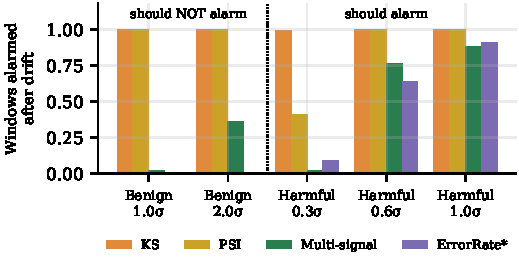
\includegraphics[width=\columnwidth]{figs/controlled.pdf}
\caption{Share of post-drift windows alarmed, mean of 20 seeds. KS and PSI cannot tell benign from harmful shift; \ours{} can.}
\label{fig:ctrl}
\end{figure}

Table~\ref{tab:ctrl} and Fig.~\ref{fig:ctrl} give the main result. In the no-drift runs, \ours{} raised no alarm in any of the 600 windows, whereas KS raised at least one false alarm in 7 of 20 runs. After a benign 1$\sigma$ shift that changed accuracy by $-0.1$ points, KS and PSI alarmed on every window, as~\cite{eck2022} observed in production; \ours{} alarmed on 2\%. For harmful shifts of 0.6$\sigma$ and 1.0$\sigma$ (accuracy $-7.8$ and $-16.6$ points), \ours{} alarmed in 90\% and 95\% of runs with a mean first-alarm delay of 1.2 and 1.0 windows---the minimum the persistence rule allows. The ablations show that voting does most of the work (OR-voting alarms on 93\% of benign windows) and persistence removes most of the remainder.

Three limits are visible. (i) At 2$\sigma$ benign shift \ours{} alarmed on 36\% of windows: tree ensembles split slightly on noise features, so very large shifts in them do move predictions. (ii) A 0.3$\sigma$ harmful shift ($-2.2$ points) is mostly missed; the label-based reference also alarms on only 9\% of these windows, as the drop is below its 5-point threshold. (iii) Pure concept drift, where $P(X)$ is unchanged, is invisible to every label-free detector (0\% detection) while ErrorRate caught all 20 runs; delayed labels remain necessary for this case.

\subsection{Real-world drift on Elec2 (Exp.~2)}
\begin{table}[t]
\caption{Elec2 stream, mean over 3 runs (82 windows of 500). Retrains and promotions are counts per run.}
\label{tab:elec2}
\centering\footnotesize\setlength{\tabcolsep}{3pt}
\begin{tabular}{lcccc}
\toprule
Strategy & Acc.\ (\%) & Worst win. & Retrains & Promoted \\
\midrule
No retraining & 67.8$\pm$0.6 & 51.1 & 0.0 & 0.0 \\
Fixed (every 4 win) & 73.9$\pm$0.5 & 52.9 & 20.0 & 15.7 \\
Fixed (every 10 win) & 73.4$\pm$0.6 & 53.8 & 8.0 & 5.0 \\
KS-triggered & 74.7$\pm$0.4 & 56.3 & 28.0 & 21.7 \\
PSI-triggered & 74.6$\pm$0.3 & 54.4 & 28.0 & 22.0 \\
\textbf{Multi-signal (ours)} & 74.4$\pm$0.3 & 55.0 & 22.7 & 17.0 \\
ErrorRate (labels)$^*$ & 73.3$\pm$0.6 & 56.4 & 17.3 & 14.0 \\
\bottomrule
\multicolumn{5}{l}{\scriptsize $^*$needs true labels at check time (supervised reference).}
\end{tabular}
\end{table}

\begin{figure}[t]
\centering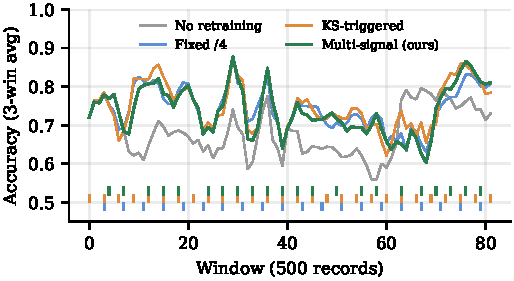
\includegraphics[width=\columnwidth]{figs/elec2_acc.pdf}
\caption{Elec2 accuracy per 500-record window (one run). Ticks at the bottom mark retrains.}
\label{fig:elec2}
\end{figure}

Table~\ref{tab:elec2} and Fig.~\ref{fig:elec2} show strong real-world degradation: the initial AutoML model scored 83.6\% on its hold-out window but only 67.8\% on the stream. Every retraining strategy recovered 5.5--6.9 points. KS and PSI fired on every window their cooldown allowed (28 of a possible 28 retrains), so on Elec2 they behave like a fixed schedule of every third window. \ours{} reached 74.4\%, within 0.3 points of KS and PSI---inside the $\pm$0.3--0.4 run-to-run spread---while using 19\% fewer retrains (22.7 versus 28), and it was 0.5 points above a fixed schedule with a similar retrain count (every 4 windows: 73.9\% with 20 retrains). The cheapest schedule (every 10 windows) lost 1.0 point against \ours. The label-based ErrorRate reference retrained less often (17.3) but scored lower, because its fixed 5-point threshold reacts only after accuracy has already dropped. At a 6\,s AutoML budget one retrain took about 7\,s of CPU.

\subsection{Live closed loop (Exp.~3)}
\begin{table}[t]
\caption{Live HTTP replay of 20{,}000 Elec2 requests.}
\label{tab:live}
\centering\footnotesize\setlength{\tabcolsep}{3pt}
\begin{tabular}{lr}
\toprule
Requests (50 rows each) & 400 \\
Latency p50 / p95 / p99 (ms) & 7.0 / 21.3 / 25.2 \\
Drift windows checked / alarms & 40 / 9 \\
Retrains promoted by gate & 6 of 9 \\
Alarm$\rightarrow$serving, median (max) & 6.5\,s (11.1\,s) \\
\quad detect / retrain / swap (s) & 0.03--0.12 / 6.2--10.9 / $<$0.04 \\
Accuracy, static v1 (same traffic) & 68.0\% \\
\textbf{Accuracy, closed loop} & \textbf{76.2\%} \\
\bottomrule
\end{tabular}
\end{table}

Table~\ref{tab:live} shows the loop running end to end on a live service. Each of the 9 alarms led to a retrain; the gate rejected 3 candidates that were not better than the serving model, and 6 new versions were hot-swapped into the running server without a restart or a failed request. Time from alarm to serving was dominated by the 6\,s AutoML budget; the pointer swap took under 40\,ms. AutoML picked XGBoost, LightGBM and extra trees at different retrains, which is why a detector tied to one model family~\cite{baier2021} would not fit this loop. Over the same 20{,}000 requests the closed loop scored 76.2\% against 68.0\% for the static initial model.

\subsection{Deployment on AWS (Exp.~4)}
\begin{table}[t]
\caption{Closed loop deployed on AWS (ap-south-1) with one SAM stack.}
\label{tab:aws}
\centering\footnotesize\setlength{\tabcolsep}{3pt}
\begin{tabular}{lr}
\toprule
Seed v1 (AutoML in Lambda, 30\,s budget) & Extra Trees \\
Traffic via API Gateway (rows 4{,}000--6{,}999) & 3{,}000 rows \\
Drift windows checked / alarms & 5 / 1 \\
Retrain in Lambda (warm AutoML + gate) & 13.0\,s \\
Candidate vs.\ serving, newest 20\% & 83.0\% vs.\ 78.8\% \\
Result & v2 (XGBoost) promoted \\
Next 3{,}000 requests served by & v2, no redeploy \\
\bottomrule
\end{tabular}
\end{table}

Table~\ref{tab:aws} repeats the loop on AWS. One \texttt{sam deploy} created the S3 bucket, both Lambda functions, the HTTP API, the hourly schedule, the CloudWatch alarm and the SNS topic. Model v1 was trained by invoking the drift function, and 3{,}000 Elec2 rows with their labels were sent through API Gateway. The next drift check raised an alarm. The function then retrained in place and the gate promoted an XGBoost model, so AutoML changed the model family on its own. The API served every following request from v2. The detector logic was identical to the local runs, while storage, scheduling and metrics were AWS services.

\section{Discussion and Limitations}
The experiments support the design goal of \ours: alarm when the model's behaviour changes, not whenever a feature moves. On data where features drift heavily but harmlessly, this removes the retrain storms that KS and PSI cause. On Elec2, where most drift is harmful, all triggered strategies end close together and the gain of \ours{} is efficiency rather than accuracy. Limitations: concept drift with unchanged inputs needs labels, so a deployment should combine \ours{} with a delayed-label error check; thresholds were set once, not tuned per dataset; AutoML with a time budget is not fully deterministic; and the AWS deployment was a short trial (6{,}000 requests), so Lambda cold-start latency and long-term cost were not measured.

\section{Conclusion}
We built and evaluated a closed-loop MLOps pipeline that joins AutoML, serverless serving, drift monitoring and gated CI/CD retraining at near-zero cloud cost, addressing gaps G1--G3. Its multi-signal detector cut false alarms on benign drift from 100\% (KS, PSI) to 2\% of windows while still catching harmful drift within about one window. A trial on AWS confirmed that the whole loop runs serverlessly. Future work: adding a delayed-label error signal as a fourth vote, adaptive thresholds, and a multi-week AWS deployment with real traffic.


\bibliographystyle{IEEEtran}
\bibliography{refs}
\end{document}
